\chapter{Core Experiments: The Canonical Setup}\label{sec:experiments}

\section{Experiments summary}\label{sec:experiments-summary}

\paragraph{Scope relative to the system model.}
The core experiments in this chapter (E2, E3) are conducted under the canonical
system model defined in Chapter~\ref{sec:methods}. In particular,
the channel remains memoryless, the noise is white, transmission is
uncoded, and relay processing is evaluated on a per-symbol basis.
Consequently, the objective of that core is to compare relay
functions under matched-model conditions rather than to address
channel estimation, sequence detection, or channels with memory.
Channel memory and channel estimation are introduced only later in
Chapter~\ref{sec:unknown-channels} as deliberate departures from the
canonical assumptions in order to study model mismatch and robustness.
Coding is introduced earlier, within this chapter, by the supplementary
coded study of Section~\ref{sec:coded-block-df}, which deliberately
departs from the uncoded, symbol-wise core to measure the
Remark~\ref{rem:df-terminology} caveat directly.

Following the single-model convention fixed in Chapter~\ref{sec:introduction}, the core of this chapter evaluates the relay strategies on the \emph{canonical setup}: a two-hop SISO link, i.i.d.\ Rayleigh fast fading on both hops, complex baseband, QPSK, uncoded BER. A supplementary coded study (Section~\ref{sec:coded-block-df}) deliberately departs from that setup within this same chapter, adding a rate-1/2 convolutional code, a block-DF relay, and an adaptive modulation-and-coding scheme. Two experiments constitute the core: the canonical relay comparison (E2) and the parameter-normalization and complexity study (E3), which together answer every canonical hypothesis (H1--H4). The principal contribution (Chapter~\ref{sec:unknown-channels}) is the unknown-channel study (E6), which tests hypothesis H5. All other departures from the canonical setup are identified as future work in Chapter~\ref{sec:discussion-and-conclusions}.
The core (E2, E3) and unknown-channel (E6) experimental configurations are summarised in the table below; the supplementary coded study's configuration is described separately in Section~\ref{sec:coded-block-df}.

Each experiment subsection reports the key results inline (BER tables and figures); supporting material and model hyperparameters are collected in the appendices (Appendices~\ref{sec:appendix-a-mathematical-notation}--\ref{sec:appendix-c-software-architecture}).

\begin{longtable}{p{0.6cm} p{2.2cm} p{2.1cm} p{3.6cm} p{3.9cm}}
\caption[Summary of experimental configurations]{Summary of core and unknown-channel experimental configurations}
\label{tab:experiment-summary}\\
\hline
\textbf{Exp.} &
\textbf{Topology} &
\textbf{Modulation} &
\textbf{Channel / Equalization} &
\textbf{Focus} \\
\hline
\endfirsthead

\hline
\textbf{Exp.} &
\textbf{Topology} &
\textbf{Modulation} &
\textbf{Channel / Equalization} &
\textbf{Focus} \\
\hline
\endhead

E2 & SISO & QPSK &
Rayleigh (canonical) &
Canonical relay comparison (H1, H2) \\
\hline

E3 & SISO & QPSK &
Rayleigh (canonical) &
Parameter normalization \& complexity (H3, H4) \\
\hline

E6 & SISO & BPSK, QPSK &
Unknown (ISI; composite; blind; partial-posterior); control: Rayleigh &
Extension: unknown-channel failure of AF/DF and learned mitigation (H5) \\
\hline

E7 & SISO & QPSK &
Rayleigh (canonical), rate-1/2 convolutional code &
Supplementary: coded block-DF against symbol-wise DF and coded-aware learned relays (Section~\ref{sec:coded-block-df}) \\
\hline

E8 & SISO & BPSK, QPSK &
All nine families above, plus the coded scenario &
Minimum relay size and the overfitting hypothesis H3, with three initializations per configuration (Section~\ref{sec:minimum-relay-size}) \\

\hline
\end{longtable}

\section{Canonical Relay Comparison (SISO, Rayleigh, QPSK)}\label{sec:siso-bpsk-performance-baseline-relay-comparison}

\textbf{Goal:} Evaluate the classical and AI-based relay strategies on the canonical setup of this thesis.

\textbf{Trials:} - \textbf{Topology:} SISO (both hops) - \textbf{Modulation scheme:} QPSK - \textbf{Channel:} i.i.d.\ Rayleigh fast fading (canonical) - \textbf{Equalizers:} One-tap coherent (per hop); no ISI equalizer needed (memoryless) - \textbf{Reported learned relay architectures (six):} Supervised (MLP, Hybrid), Generative (VAE), Sequence (Transformer, Mamba-S6, Mamba-2 SSD) - \textbf{NN activation:} ReLU hidden, tanh output

\textbf{Conclusion:} On the canonical Rayleigh channel, AI relays match but do not surpass symbol-wise DF: DF achieves the lowest or tied-lowest BER at essentially every SNR point, including the low-SNR regime, while the best neural relays (MLP, Hybrid, VAE) track it within statistical uncertainty and clearly outperform AF. This confirms H1 (AI relays beat AF at low SNR) and H2 (DF dominance at $\geq 6$ dB with zero trainable parameters) on the canonical channel.

\subsection{Results Tables}\label{sec:results-tables}

\begingroup\footnotesize
\begin{longtable}[]{@{}lccccccccc@{}}
\caption[BER on the canonical setup]{BER on the canonical setup: QPSK over i.i.d.\ Rayleigh fast fading, SISO on both hops, uncoded, $10\times10{,}000$ bits per SNR point. ``DF th.'' is the closed-form two-hop composition of Eq.~\ref{eq:df-ber-rayleigh} (Section~\ref{sec:rayleigh-two-hop-df-ber}), included for direct comparison against the measured DF column. Column abbreviations: Transf.\ is the Transformer relay, Mamba2 the Mamba-2 SSD relay}\label{tbl:table2}\tabularnewline
\toprule\noalign{}
SNR (dB) & AF & DF & DF th. & MLP & Hybrid & VAE & Transf. & Mamba-S6 & Mamba2 \\
\midrule\noalign{}
\endfirsthead
\toprule\noalign{}
SNR (dB) & AF & DF & DF th. & MLP & Hybrid & VAE & Transf. & Mamba-S6 & Mamba2 \\
\midrule\noalign{}
\endhead
\bottomrule\noalign{}
\endlastfoot
0 & 0.4076 & 0.3337 & 0.3333 & 0.3349 & \textbf{0.3329} & 0.3359 & 0.4014 & 0.4071 & 0.4032 \\
4 & 0.3129 & \textbf{0.2219} & 0.2216 & 0.2233 & 0.2220 & 0.2254 & 0.2758 & 0.2812 & 0.2772 \\
8 & 0.1852 & \textbf{0.1218} & 0.1203 & 0.1229 & 0.1220 & 0.1235 & 0.1424 & 0.1448 & 0.1416 \\
12 & 0.0822 & 0.0580 & 0.0560 & 0.0586 & \textbf{0.0579} & 0.0589 & 0.0628 & 0.0637 & 0.0621 \\
16 & 0.0309 & \textbf{0.0245} & 0.0239 & 0.0247 & \textbf{0.0245} & 0.0247 & 0.0260 & 0.0259 & 0.0251 \\
20 & 0.0110 & \textbf{0.0097} & 0.0098 & 0.0099 & \textbf{0.0097} & \textbf{0.0097} & 0.0101 & 0.0100 & 0.0098 \\
\end{longtable}
\endgroup

Two features of Table~\ref{tbl:table2} deserve comment. First, symbol-wise DF tracks the closed form (the ``DF th.'' column above): reading the abscissa as $E_s/N_0$ and converting to $E_b/N_0$ for QPSK ($k=2$, so $3.01$~dB lower), the two-hop expression $2P(1-P)$ with $P=\tfrac12\bigl(1-\sqrt{\bar\gamma/(1+\bar\gamma)}\bigr)$ gives agreement to within a few percent relative error at every tabulated point ($1.1\%$ at 20~dB, $2.4\%$ at 16~dB, worst case $3.5\%$ at 12~dB, each recomputable from the four-decimal values as printed), which validates the simulator end to end against the analysis of Section~\ref{sec:rayleigh-two-hop-df-ber}. Figure~\ref{fig:fig10} plots this closed form alongside the measured curves, together with the single-hop floor $P$ itself -- the BER a genie that recovered hop~1 perfectly would still incur on hop~2 -- which no relay may cross and none does at any SNR.

Second, the relays divide by family rather than by paradigm. The three feedforward relays, the MLP, the Hybrid and the VAE, are statistically indistinguishable from DF from 4~dB upward and from each other throughout; the VAE reaches $0.00972$ at 20~dB, matching DF exactly at the resolution of this budget. The two sequence models are the ones that separate, trailing by roughly $0.07$ in BER at 0~dB before converging by 16~dB. Capacity is not the explanation, since the sequence models are the larger of the two groups; the memoryless channel simply offers no temporal structure for their inductive bias to exploit, a reading the equal-parameter comparison of Section~\ref{sec:parameter-normalization-complexity-trade-off} tests directly and confirms.

Two comments on Table~\ref{tbl:table2}. First, symbol-wise DF is the best or tied-best relay at every tabulated point, and the learned relays sit within a few thousandths of it from 4~dB upward: on a matched, known channel the learned relay matches DF rather than beating it, at 169 parameters against DF's none. This is H2, and it is the result the rest of the thesis is measured against. Second, the two sequence models trail the feedforward relays at low SNR (0~dB row of Table~\ref{tbl:table2}) and converge with them by 16~dB, so their extra capacity buys nothing on a memoryless channel; Section~\ref{sec:parameter-normalization-complexity-trade-off} separates that from the parameter-count confound.

\paragraph{Why QPSK and not BPSK.} QPSK places one bit on each axis the Rayleigh coefficient acts in, carries two bits per symbol, and is processed by the I/Q-split relays without modification, which makes it the constellation that exercises the complex-signal processing this thesis studies. Coherent BPSK over the same complex channel would be entirely valid --- after channel-phase removal the whole BPSK component lies on the real decision axis, so projecting onto it discards no signal energy --- and the choice here is one of experimental design rather than of correctness (Section~\ref{sec:evaluated-configurations}). One consequence must be kept in view when reading these BER figures against BPSK closed forms: the SNR axis here is $E_s/N_0$, and QPSK carries two bits per symbol, so a given abscissa corresponds to an $E_b/N_0$ that is $3.01$~dB lower than the same number on a BPSK axis. The constellations are not on a common axis and their error rates are not directly comparable.

\subsection{Results Figures}\label{sec:results-figures-1}

\begin{figure}[htbp]
\centering
\pandocbounded{\includegraphics[width=\linewidth,height=0.8\textheight,keepaspectratio]{results/canonical_qpsk_rayleigh_ci.png}}
\caption[The canonical setup]{The canonical setup: QPSK over i.i.d.\ Rayleigh fast fading, BER vs.\ $E_s/N_0$ for the eight relays of Table~\ref{tbl:table2}, with 95\% confidence intervals, plus two theoretical reference curves: ``DF (theory)'' (dashed), the closed-form two-hop composition, which the measured DF curve tracks closely, within a few percent relative error everywhere (worst case $3.6\%$, at 12~dB); and the ``single-hop floor'' (dotted), the BER a genie that recovered hop~1 perfectly would still incur on hop~2 -- a reference floor for this fixed-rate, fixed-power relay chain. AF is uniformly worst; symbol-wise DF and the feedforward learned relays are indistinguishable from 4~dB upward; the two sequence models trail at low SNR and converge by 16~dB}\label{fig:fig10}
\end{figure}

\section{Parameter Normalization \& Complexity Trade-off}\label{sec:parameter-normalization-complexity-trade-off}

This study tests H3 (complexity versus BER) and H4 (architecture convergence at an equal parameter budget) on the canonical setup.

\textbf{Goal:} Isolate architectural inductive biases from parameter count effects and characterize the complexity-performance trade-off for relay denoising.

\textbf{Trials:} - \textbf{Topology:} SISO (both hops) - \textbf{Modulation scheme:} QPSK - \textbf{Channel:} i.i.d.\ Rayleigh fast fading (canonical) - \textbf{Equalizers:} One-tap coherent (per hop); no ISI equalizer needed (memoryless) - \textbf{NN architecture:} All normalized to \textasciitilde3,000 parameters, plus original sizes (169 to 26K) - \textbf{NN activation:} ReLU hidden, tanh output

\textbf{Conclusion:} A minimal 169-parameter MLP matches models roughly 140$\times$ larger, and no larger model evaluated here improves on it; whether the curve eventually turns upward, and whether overfitting would be the reason, is not tested by \emph{these} experiments (Section~\ref{sec:capacity-and-overfitting}). It is tested by the size sweep of Section~\ref{sec:minimum-relay-size}, which replicates every configuration across three initializations and finds no upward arm above the initialization spread. At an equal budget of 3,000 parameters the gap between feedforward and sequence architectures is strongly SNR-dependent: it falls monotonically from $17.4\%$ at 0~dB to $4.1\%$ at 20~dB (Table~\ref{tbl:table8}). Parameter count therefore accounts for the comparison at high SNR, where the choice of model is nearly irrelevant, but not at low SNR, where the six equal-sized models separate cleanly into a feedforward group tracking DF and a sequence group tracking AF. Since all six carry the same budget, that separation is not explained by capacity; it is attributable to the remaining differences between the models, of which architecture is the most salient but not the only one, since depth, width, state dimension and window size were adjusted to meet the budget (Table~\ref{tbl:table28}). The generative VAE falls inside the feedforward group at every SNR rather than apart from it, ending at $0.0101$ against MLP-3K's $0.0099$, and it is ahead of all three sequence models from 0 to 16~dB; the generative paradigm is therefore not a handicap at this budget (Section~\ref{sec:generative-vs.-discriminative-paradigms-for-relay-processing}).

\subsection{Results Tables}\label{sec:results-tables-2}

\begingroup\footnotesize
\begin{longtable}[]{@{}lcccccccc@{}}
\caption[Equal-parameter-budget comparison at 3K]{Equal-parameter-budget comparison on the canonical setup (QPSK over Rayleigh). All learned columns are the $\sim$3{,}000-parameter variants; every learned model is scaled to approximately 3{,}000 parameters, so parameter count is removed as an explanation for the residual differences; width, depth, state dimension and window size still co-vary with architecture (Table~\ref{tbl:table28}). AF and DF are the unparameterized references. Column abbreviations: Transf.\ is the Transformer relay, Mamba2 the Mamba-2 SSD relay}\label{tbl:table8}\tabularnewline
\toprule\noalign{}
SNR (dB) & MLP & Hybrid & VAE & Transf. & Mamba-S6 & Mamba2 & AF & DF \\
\midrule\noalign{}
\endfirsthead
\toprule\noalign{}
SNR (dB) & MLP & Hybrid & VAE & Transf. & Mamba-S6 & Mamba2 & AF & DF \\
\midrule\noalign{}
\endhead
\bottomrule\noalign{}
\endlastfoot
0 & 0.3361 & 0.3391 & 0.3424 & 0.4068 & 0.4007 & 0.4001 & 0.4076 & \textbf{0.3337} \\
4 & 0.2244 & 0.2271 & 0.2291 & 0.2818 & 0.2751 & 0.2742 & 0.3129 & \textbf{0.2219} \\
8 & 0.1229 & 0.1229 & 0.1267 & 0.1458 & 0.1406 & 0.1405 & 0.1852 & \textbf{0.1218} \\
12 & 0.0586 & 0.0580 & 0.0604 & 0.0640 & 0.0620 & 0.0622 & 0.0822 & \textbf{0.0580} \\
16 & 0.0247 & \textbf{0.0245} & 0.0251 & 0.0259 & 0.0250 & 0.0251 & 0.0309 & \textbf{0.0245} \\
20 & 0.0099 & \textbf{0.0097} & 0.0101 & 0.0100 & 0.0097 & 0.0098 & 0.0110 & \textbf{0.0097} \\
\end{longtable}
\endgroup

\begin{figure}[htbp]
\pandocbounded{\includegraphics[width=\linewidth,height=0.8\textheight,keepaspectratio]{results/normalized_3k_rayleigh_ber.png}}
\caption[Equal-parameter-budget BER (3K), QPSK/Rayleigh]{BER vs $E_s/N_0$ for all relay variants normalised to $\approx$3{,}000 parameters, QPSK over Rayleigh fading. AF and DF (dashed) are the unparameterised references. Shaded bands show 95\% confidence intervals for the learned relays. The feedforward group (MLP-3K, Hybrid-3K, VAE-3K) tracks DF across the full range; the sequence models (Transformer-3K, Mamba-3K, Mamba2-3K) converge with them only at high SNR}\label{fig:fig-3k-ber}\end{figure}

\section{Minimum Relay Size Across Channel Families}\label{sec:minimum-relay-size}

The complexity study of Section~\ref{sec:parameter-normalization-complexity-trade-off} establishes that no evaluated model improves on the 169-parameter MLP, but leaves two questions open: how far \emph{below} 169 parameters the relay can be taken, and whether the answer is a property of the architecture or of the channel. This section answers both by sweeping relay size downward on every channel family used in this thesis.

\textbf{Goal:} Locate the smallest relay that costs nothing measurable against the thesis's own published relay, per channel, and determine which architectural axis --- window, depth or width --- sets that floor.

\textbf{Trials:} - \textbf{Topology:} SISO, two hops, hop~2 per each channel family's own convention (AWGN or coherently-compensated Rayleigh) - \textbf{Modulation scheme:} BPSK or QPSK, per channel, as used elsewhere in this thesis - \textbf{Channels:} the nine families of Chapters~\ref{sec:experiments} and~\ref{sec:unknown-channels}, plus the coded scenario of Section~\ref{sec:coded-block-df} - \textbf{Comparators:} symbol-wise DF where the channel is memoryless, Viterbi/MLSE where it has memory, block DF for the coded scenario; each channel additionally compared against its own published relay (MLP-169, or MLP-756 coded) - \textbf{Relay architecture:} window $\in\{1,3,5,7\}$, depth $\in\{1,2,3\}$, width from 1 to 48 - \textbf{Replication:} three independent initializations per configuration, each configuration held to its worst - \textbf{Metric:} additional SNR required to reach a given BER

\textbf{Conclusion:} The floor is set by channel memory, not by parameter count, and it is far lower than 169 parameters only where the channel is memoryless. Table~\ref{tbl:table-minsize} gives the smallest configuration meeting a range of degradation budgets against each scenario's own published relay. At zero degradation, three of the five memoryless channels are matched by four parameters --- a single hidden unit with no window, $42\times$ smaller than MLP-169 --- whereas the three-tap channels require 73 to 145 parameters, only $1.2\times$ to $2.3\times$ smaller. Reading the window column rather than the parameter column explains why: every memoryless row settles at window~1 and every three-tap row needs window~5 or~7 until a full decibel of degradation is permitted. Figure~\ref{fig:minsize-crossover} shows the same effect directly --- widening the window is worth $8$ to $11$~dB on the three-tap channels and nothing at all on the memoryless ones --- and Figure~\ref{fig:minsize-budget} plots the size required against the degradation the designer is willing to concede. Depth was varied from one to three hidden layers and improved no configuration; where a two-layer network matched, a single layer matched at fewer parameters. The complexity question is therefore not "how many parameters" but "how much window", and the answer is fixed by the channel's impulse response rather than by the architecture. Section~\ref{sec:complexity-curve-turn} takes up what this implies for the overfitting hypothesis H3, and reports the across-initialization spread that bounds the resolution of these figures.

The full budget-by-budget table is Table~\ref{tbl:table-minsize} in Appendix~\ref{sec:appendix-f-minimum-size}, together with the two figures that show the window effect directly (Figures~\ref{fig:minsize-crossover} and~\ref{fig:minsize-budget}).

\section{Coded Block-DF: Measuring the Remark~\ref{rem:df-terminology} Caveat}\label{sec:coded-block-df}

\paragraph{A note on constellation scope.} The canonical and coded-study fixed-MCS relay-decoding comparisons of this thesis (block-DF vs.\ the learned relay at a fixed code rate and constellation) are conducted on QPSK throughout; the unknown-channel study's relay comparisons mainly use BPSK (Chapter~\ref{sec:unknown-channels}), with one exception (Section~\ref{sec:qpsk-unknown-channel}) that repeats the unknown-ISI relay comparison with QPSK in place of BPSK. 16-QAM is not studied as a relay-architecture question (Section~\ref{sec:modulation-schemes}): it does appear as one rung of the modulation-and-coding ladder that the link-adaptation study of Section~\ref{sec:coded-rate-adaptation} selects from, and that study does compare the block-DF and denoise-only relay strategies at 16-QAM rungs (e.g.\ Table~\ref{tbl:table42}), but the object of study there is the \emph{rate-and-modulation choice} rather than the relay's ability to process a denser constellation. Nothing in that study rests on how a learned relay handles four levels per axis, which is the question left to future work.

Remark~\ref{rem:df-terminology} draws a distinction the rest of this thesis relies on: the DF baseline used everywhere here is \emph{symbol-wise} (uncoded, per-symbol hard slicing), not the \emph{block} DF of the information-theoretic relay-channel literature, and the remark explicitly cautions that "the reported DF results should not be read as bounds on coded block-DF performance." That caveat was asserted, not measured. This section measures it: a practical finite-length coded block-DF relay, built from a rate-1/2 convolutional code and a soft-decision Viterbi decoder, added as a supplementary study on the canonical channel rather than as a revision of the core comparison above.

\textbf{Setup.} A standard rate-1/2 convolutional code (constraint length $K$, $2^{K-1}$ trellis states, zero-tail terminated per 200-information-bit frame) is applied before QPSK modulation on the canonical Rayleigh channel; \texttt{CodedDecodeAndForwardRelay} decodes the full frame at the relay via soft-decision Viterbi (squared-distance branch metric on the coherently-compensated I/Q samples), then re-encodes and re-modulates a fresh, clean codeword before forwarding -- genuine block DF, as opposed to the per-symbol slicing used elsewhere in this thesis. Two coded-aware learned relays are trained on the same task for comparison: a windowed 756-parameter MLP classifier (window 21, $\approx$5$\times K$ for $K=3$) and the Mamba-S6 architecture already used in Table~\ref{tbl:table2} (24,084 parameters at this configuration), both predicting the transmitted QPSK symbol from a window of noisy coded observations with no explicit knowledge of the code. All results use the thesis-standard budget of 100 trials $\times$ 100,000 information bits per SNR point.

\begin{longtable}[]{@{}lcccccc@{}}
\caption[Coded block-DF vs.\ uncoded DF and coded-aware learned relays]{Coded block-DF vs.\ uncoded symbol-wise DF and coded-aware learned relays, canonical QPSK/Rayleigh, rate-1/2 $K{=}3$ code. ``coded-AF'' forwards the noisy codeword unmodified (the relay does not decode), isolating the code's own gain from any relay intelligence}\label{tbl:table34}\tabularnewline
\toprule\noalign{}
SNR (dB) & uncoded DF & coded AF & coded DF & MLP-coded & Mamba-coded \\
\midrule\noalign{}
\endfirsthead
\toprule\noalign{}
SNR (dB) & uncoded DF & coded AF & coded DF & MLP-coded & Mamba-coded \\
\midrule\noalign{}
\endhead
\bottomrule\noalign{}
\endlastfoot
0 & \textbf{0.3337} & 0.4902 & 0.4204 & 0.4439 & 0.4505 \\
4 & \textbf{0.2216} & 0.4468 & 0.2229 & 0.2974 & 0.3214 \\
8 & 0.1205 & 0.2722 & \textbf{0.0638} & 0.1010 & 0.1174 \\
12 & 0.0560 & 0.0539 & \textbf{0.0154} & 0.0214 & 0.0226 \\
16 & 0.0239 & 0.0099 & 0.0042 & 0.0045 & \textbf{0.0041} \\
20 & 0.0098 & 0.0020 & 0.0014 & 0.0011 & \textbf{0.0010} \\
\end{longtable}

\begin{figure}[htbp]
\pandocbounded{\includegraphics[width=\linewidth,height=0.8\textheight,keepaspectratio]{results/coded_df_ber.png}}
\caption[Coded block-DF vs uncoded DF and learned relays, BER vs SNR]{BER vs $E_s/N_0$ for coded block-DF, uncoded symbol-wise DF, and the two coded-aware learned relays (MLP and Mamba), canonical QPSK/Rayleigh, rate-1/2 $K{=}3$. Coding hurts below the measured crossover (between 4 and 8~dB for this code, decoder, frame and SNR convention) and helps decisively above it; the learned relays close on coded-DF only at the top of the sweep}\label{fig:fig-coded-df-ber}\end{figure}

Two findings, reported as measured rather than smoothed toward either a "coding always helps" or a "the learned relay wins" narrative:

\textbf{The caveat holds precisely where it should, and no further.} At equal $E_s/N_0$, coded block-DF beats uncoded symbol-wise DF decisively from 8~dB upward -- a $5.7\times$ reduction in BER at 16~dB, $7.2\times$ at 20~dB -- closing the gap the remark left open. Those factors are the right comparison for a detection question but the wrong one for a link budget, because the rate-1/2 code halves the information carried per channel use; Section~\ref{sec:coded-latency-throughput} redoes the comparison at equal throughput and the advantage largely disappears. But below roughly 6~dB, coding \emph{hurts} even on the favourable axis: both coded AF and coded DF are worse than plain uncoded DF at 0 and 4~dB. This is the measured crossover for this configuration, not an artifact: for this finite-length code, decoder, frame, modulation and SNR convention the coded and uncoded curves cross between 4 and 8~dB, and below that crossover a fixed-rate code produces decoding errors that cluster and propagate across the trellis, which a memoryless per-symbol slicer cannot do. The caveat is real, but it cuts both ways -- coded block-DF is a strictly stronger baseline only above its own threshold, which itself has to be measured, not assumed.

\textbf{At low-to-mid SNR the classical decoder is far ahead, and the learned relay's extra capacity buys nothing.} Unlike the canonical memoryless channel of Table~\ref{tbl:table2}, where Section~\ref{sec:parameter-normalization-complexity-trade-off} found "the memoryless channel simply offers no temporal structure for [the sequence models'] inductive bias to exploit," a convolutional code \emph{is} genuine temporal structure. It does not rescue the learned relays where the code is doing the most work: both are far behind coded-DF at 4--8~dB, and the 32$\times$-larger Mamba-S6 relay shows no clear advantage over the 756-parameter MLP there, being worse at 4--8~dB (Table~\ref{tbl:table34}). Giving the sequence model a task with real memory to exploit therefore does not overturn the thesis's minimal-capacity finding (H3): extra capacity still buys no reliable advantage over the minimal architecture.

\textbf{At high SNR the ordering reverses, and it is not noise.} The differences at 16--20~dB in Table~\ref{tbl:table34} are small in absolute terms, and an earlier version of this section dismissed them as trial-to-trial variation. That was wrong, and the correction is worth stating explicitly because it changes the conclusion. Re-measuring those two points with \emph{paired} trials -- every relay driven by identical information bits and identical hop-1/hop-2 fading realizations within each trial, so the channel-draw variance that dominates an unpaired comparison cancels in the per-trial difference -- and testing with the Wilcoxon signed-rank test used elsewhere in this thesis gives Table~\ref{tbl:table37}. At 20~dB both learned relays beat coded-DF in essentially every one of 100 paired trials ($p<10^{-4}$). At 16~dB the result splits by architecture: Mamba-coded wins (68 of 100 trials) while the MLP significantly \emph{loses} (23 of 100), both at $p<10^{-4}$. The effects are real in both directions, and no single sentence of the form ``the learned relay beats/does not beat Viterbi'' describes them.

\begin{longtable}[]{@{}lccccc@{}}
\caption[Paired re-measurement of the high-SNR points]{Paired re-measurement of the two high-SNR points of Table~\ref{tbl:table34}, 100 paired trials $\times$ 100{,}000 information bits. ``Diff'' is the mean per-trial BER difference against coded-DF (negative favours the learned relay); ``W/L'' counts trials won/lost; $p$ is Wilcoxon signed-rank}\label{tbl:table37}\tabularnewline
\toprule\noalign{}
SNR & Relay & BER & Diff vs.\ coded-DF & W/L & $p$ \\
\midrule\noalign{}
\endfirsthead
\toprule\noalign{}
SNR & Relay & BER & Diff vs.\ coded-DF & W/L & $p$ \\
\midrule\noalign{}
\endhead
\bottomrule\noalign{}
\endlastfoot
16 dB & coded-DF & 0.004245 & --- & --- & --- \\
 & MLP-coded & 0.004437 & $+0.000192$ & 23/77 & $<10^{-4}$ \\
 & Mamba-coded & \textbf{0.004124} & $-0.000121$ & 68/32 & $<10^{-4}$ \\
\hline
20 dB & coded-DF & 0.001362 & --- & --- & --- \\
 & MLP-coded & 0.001066 & $-0.000295$ & 99/1 & $<10^{-4}$ \\
 & Mamba-coded & \textbf{0.000967} & $-0.000395$ & 100/0 & $<10^{-4}$ \\
\end{longtable}

\textbf{This is not a learned relay out-decoding Viterbi, and the mechanism says why.} Viterbi is the maximum-likelihood \emph{sequence} decoder for a known code on a known channel, so a learned decoder beating it at its own task would be a surprising claim requiring more than a BER table. It is not what happens here. Instrumenting the relay output directly (Table~\ref{tbl:table38}) shows coded-DF is the \emph{better} decoder by a wide margin: it puts roughly $2.1\times$ \emph{fewer} symbol errors on the air than the learned relay at both SNRs, exactly as the optimality result predicts. What separates them is what happens to those errors afterwards. Coded-DF decodes and then \emph{re-encodes}, so a frame it gets wrong leaves the relay as a different but perfectly \emph{valid} codeword: the code's redundancy has been spent and then regenerated around the error, and the destination's decoder has no way to detect or repair it. The learned relay never re-encodes, so its (more numerous) mistakes remain isolated bad symbols inside an otherwise-valid codeword, and the destination still holds the redundancy needed to fix them. Only 16--25\% of coded-DF's relay errors are repaired downstream against 58--73\% of the learned relay's. That also explains the SNR-dependent split above: at 16~dB the $2.1\times$ raw-error penalty still outweighs the repair advantage for the MLP, and by 20~dB it no longer does.

\begin{longtable}[]{@{}lccccc@{}}
\caption[Where the errors go: relay output versus destination output]{Where the errors go, 100 trials $\times$ 500 frames. ``Relay symbol ER'' counts symbols the relay put on the air that differ from the transmitted ones; ``repaired'' is the fraction of those that do not survive the destination's decoder. The oracle relay forwards the clean codeword and so isolates the hop-2-only floor}\label{tbl:table38}\tabularnewline
\toprule\noalign{}
SNR & Relay & Relay symbol ER & Repaired & Final BER \\
\midrule\noalign{}
\endfirsthead
\toprule\noalign{}
SNR & Relay & Relay symbol ER & Repaired & Final BER \\
\midrule\noalign{}
\endhead
\bottomrule\noalign{}
\endlastfoot
16 dB & coded-DF & \textbf{0.00505} & 15.7\% & 0.004257 \\
 & MLP-coded & 0.01065 & \textbf{57.9\%} & 0.004487 \\
 & oracle & --- & --- & 0.002140 \\
\hline
20 dB & coded-DF & \textbf{0.00182} & 24.7\% & 0.001369 \\
 & MLP-coded & 0.00385 & \textbf{73.0\%} & 0.001039 \\
 & oracle & --- & --- & 0.000668 \\
\end{longtable}

\paragraph{Does a stronger code help?} The $K{=}3$ code used above is deliberately small. Sweeping the constraint length to $K\in\{5,7\}$ on the same QPSK/Rayleigh link does \emph{not} improve matters: the larger-$K$ codes are worse than $K{=}3$ across 0--8~dB, a sharper error-propagation cliff for the bigger trellis, and by 20~dB all three are within trial-to-trial noise of one another (values $0.0014$, $0.0015$, $0.0012$). Within this frame length and trial budget, the relay's re-encoding liability is therefore not something a stronger code repairs; the full sweep is available in \url{results/coded_df_experiment.json}.

\paragraph{Does reliable decoding remove it?} Remark~\ref{rem:df-terminology} defines block-DF with ``a strong (ideally capacity-achieving) channel code'', which the measurements above do not approach: at $20$~dB the destination fails on $20.23\%$ of frames under coded-DF and on $10.58\%$ even under an \emph{oracle} relay forwarding the clean codeword, so one frame in ten is lost for reasons unrelated to the relay. Since the liability tracks the relay's frame-error rate rather than the code family behind it, the link is extended up the SNR axis, code fixed, until decoding is reliable (Table~\ref{tbl:table44}); two learned relays are run, one on the recipe above and one retrained on $5$--$30$~dB, which brackets three of the four evaluated points and leaves only the $32$~dB reading as a mild, $2$~dB extrapolation, so no high-SNR reading rests on a large train/test mismatch.

\begingroup\footnotesize
\begin{longtable}[]{@{}lccccc@{}}
\caption[Block-DF into the reliable-decoding regime]{Block-DF into the reliable-decoding regime: the rate-1/2 $K{=}3$ code and canonical QPSK/Rayleigh link of Table~\ref{tbl:table34}, extended up the SNR axis, $100$ trials $\times$ $1{,}000$ frames ($20{,}000{,}000$ information bits) per point. ``MLP (5/10/15)'' uses that table's training recipe; ``MLP (5--30)'' is the same architecture retrained on $5$--$30$~dB, bracketing all but the $32$~dB point, hence a different instance whose $20$~dB entry need not reproduce it. Bold marks the best \emph{relay} in each row (both marked where they tie); the oracle forwards the clean codeword and is the single-decode floor they are measured against, not a competitor}\label{tbl:table44}\tabularnewline
\toprule\noalign{}
SNR (dB) & coded-DF & MLP (5/10/15) & MLP (5--30) & oracle & coded-DF FER \\
\midrule\noalign{}
\endfirsthead
\toprule\noalign{}
SNR (dB) & coded-DF & MLP (5/10/15) & MLP (5--30) & oracle & coded-DF FER \\
\midrule\noalign{}
\endhead
\bottomrule\noalign{}
\endlastfoot
20 & 0.001378 & \textbf{0.001064} & 0.001092 & 0.000703 & 0.1998 \\
24 & 0.000485 & \textbf{0.000308} & 0.000318 & 0.000253 & 0.0804 \\
28 & 0.000187 & \textbf{0.000105} & 0.000105 & 0.000092 & 0.0324 \\
32 & 0.000069 & \textbf{0.000037} & \textbf{0.000037} & 0.000034 & 0.0122 \\
\end{longtable}
\endgroup

\begin{figure}[htbp]
\pandocbounded{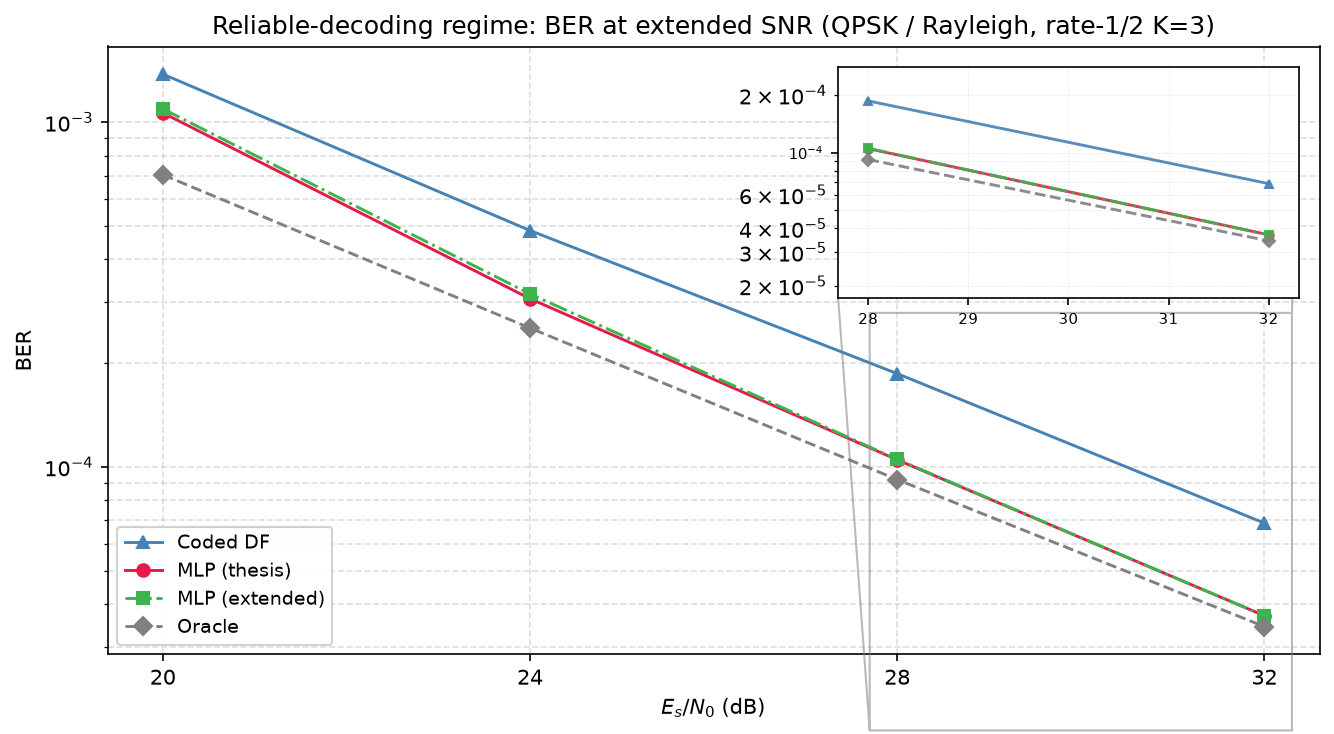
\includegraphics[width=\linewidth,height=0.8\textheight,keepaspectratio]{results/coded_reliable_regime.png}}
\caption[Reliable-decoding regime: BER at extended SNR]{BER vs $E_s/N_0$ at extended SNR ($20$--$32$~dB), rate-1/2 $K{=}3$ QPSK/Rayleigh. Coded DF's BER remains near twice the oracle floor at every point; the retrained learned relay (MLP 5--30~dB) closes on that floor monotonically and reaches statistical parity with it at 32~dB, demonstrating that the high-SNR reversal survives into the reliable-decoding regime}\label{fig:fig-reliable-regime}\end{figure}

\textbf{The liability does not dissolve.} Across $20$--$32$~dB coded-DF's frame-error rate falls $16.3\times$ ($0.1998$ to $0.0122$), yet its BER stays near twice the oracle floor with no trend at all ($1.96$, $1.92$, $2.03$, $2.00$; the scatter is trial noise, the absence of a downward slope is the point), while the retrained learned relay (MLP $5$--$30$) closes on that floor ($1.55$, $1.26$, $1.15$, $1.08$) and reaches statistical parity with it by $32$~dB ($636$ against $607$ frame errors in $100{,}000$, $z=+0.8$) while still beating coded-DF there ($z=+13.7$). The cause is structural, not code strength: block-DF decodes once per hop, so two independent frame-error events accumulate and neither decoder repairs the other's, whereas denoising leaves a single decoding operation at the destination. The reversal is thus no artefact of a weak code or short frame; it survives, and relatively widens, as decoding becomes reliable. One limit stays out of reach: driving per-hop failure to zero makes the sum of two vanishing terms vanish, so a capacity-achieving code at long blocklength would recover the floor. No operating point here does: even at $32$~dB the oracle's own decode -- one hop's worth, by construction, and equal to the other hop's by the link's symmetry -- still fails on $0.6\%$ of frames.

\subsection{Soft-Decision Relaying, and What the Liability Actually Is}\label{sec:coded-soft-decision}

The mechanism of Table~\ref{tbl:table38} suggests an obvious repair. If the trouble with block-DF is that it commits to a codeword, replace the commitment with soft information: run BCJR (forward-backward MAP) at the relay instead of Viterbi and forward the posterior-mean symbol per trellis step, so a symbol the relay is unsure of is shrunk toward the origin rather than asserted. The same idea applies to the learned relay, whose softmax already carries a posterior it was throwing away: forwarding $\sum_k p_k s_k$ instead of $\arg\max_k p_k$ costs nothing, needs no retraining, and reuses the identical weights, so any difference isolates the read-out rule alone. Table~\ref{tbl:table39} evaluates both against their hard counterparts and against an oracle relay that forwards the clean codeword, on paired trials.

\begin{longtable}[]{@{}lccccc@{}}
\caption[Soft- versus hard-decision relaying on the coded link]{Soft- versus hard-decision relaying, canonical QPSK/Rayleigh, rate-1/2 $K{=}3$, 100 paired trials $\times$ 100{,}000 information bits. The MLP hard/soft pair shares one set of trained weights and differs only in the read-out. The oracle relay forwards the clean codeword, giving the hop-2-only floor. Both block-DF variants are marked at 8~dB, where they are a statistical tie}\label{tbl:table39}\tabularnewline
\toprule\noalign{}
SNR (dB) & hard block-DF & soft block-DF & MLP hard & MLP soft & oracle \\
\midrule\noalign{}
\endfirsthead
\toprule\noalign{}
SNR (dB) & hard block-DF & soft block-DF & MLP hard & MLP soft & oracle \\
\midrule\noalign{}
\endhead
\bottomrule\noalign{}
\endlastfoot
0 & 0.4208 & \textbf{0.4150} & 0.4443 & 0.4343 & 0.3022 \\
4 & 0.2231 & \textbf{0.2218} & 0.2969 & 0.2761 & 0.1278 \\
8 & \textbf{0.0636} & \textbf{0.0636} & 0.1008 & 0.0878 & 0.0327 \\
12 & \textbf{0.01537} & 0.01537 & 0.02142 & 0.01768 & 0.00768 \\
16 & 0.004222 & 0.004222 & 0.004403 & \textbf{0.003633} & 0.002105 \\
20 & 0.001354 & 0.002348$^{\dagger}$ & 0.001056 & \textbf{0.000912} & 0.000682 \\
\multicolumn{6}{l}{\footnotesize $^{\dagger}$Nominal-noise-variance run; miscalibrated at high SNR (see text below). The variance-corrected figure is $0.001376$, a statistical tie with hard block-DF's $0.001375$.} \\
\end{longtable}

\begin{figure}[htbp]
\centering
\pandocbounded{\includegraphics[width=\linewidth]{results/coded_soft_decision.png}}
\caption[Soft- versus hard-decision relaying: BER curves]{Soft- versus hard-decision relaying on the coded link (canonical QPSK/Rayleigh, rate-1/2 $K{=}3$, 100 paired trials). The soft MLP (posterior mean) tracks below the hard MLP at every SNR, with the largest gain visible at mid-to-high SNR where the relay's residual uncertainty is most useful to the destination decoder. The two block-DF variants (hard Viterbi, soft BCJR) converge at high SNR and are never separated by a reliable margin, confirming that the liability is consuming the code's redundancy at the relay rather than hard quantization per se. The oracle relay (dashed) is the hop-2-only floor}\label{fig:fig57}
\end{figure}

\textbf{Soft read-out helps the learned relay everywhere} (Figure~\ref{fig:fig57}). At every SNR the posterior mean beats the argmax, on identical weights (columns 3--4 of Table~\ref{tbl:table39}). The gain is largest exactly where the mechanism predicts, since a relay that reports its uncertainty gives the destination's decoder more to work with than one that reports a confident guess. It is enough to change a verdict: at 16~dB the hard MLP significantly \emph{loses} to block-DF (19 wins, 80 losses and one tie) while the soft MLP significantly \emph{beats} it (100 wins, no losses), and at 20~dB the soft relay comes within $0.00023$ of the oracle floor that no relay in this fixed-rate, fixed-power chain can pass.

\textbf{Soft block-DF does not rescue block-DF, and that is the more interesting result.} The prediction going in was that BCJR would combine the code-aware cleanup of Viterbi with the repairability of a non-committing relay, and therefore beat both. It does not. It edges hard block-DF at 0--4~dB, ties it from 8--16~dB, and at 20~dB is clearly worse (Table~\ref{tbl:table39}, losing all 100 paired trials). The 20~dB degradation turns out to be a calibration artefact rather than a property of soft forwarding: the relay is given the \emph{nominal} noise variance, but post-equalization Rayleigh noise has variance $1/(2\gamma|h|^2)$, so at high SNR, where the nominal value is small, BCJR becomes badly overconfident on deep-fade symbols. Viterbi is structurally immune, its squared-distance metric being invariant to any uniform scaling of the assumed variance. Deliberately inflating the assumed variance confirms this directly: at 20~dB a factor of two removes the entire gap ($0.002404 \to 0.001376$), and every larger factor up to $100\times$ holds there.

What that correction exposes is the substantive point. Even properly calibrated, soft block-DF only \emph{ties} hard block-DF ($0.001376$ against $0.001375$ at 20~dB; $0.004255$ against $0.004255$ at 16~dB) -- it never beats it. The reason is that at high SNR the BCJR posteriors saturate, so the posterior mean degenerates to the constellation point and soft block-DF reproduces Viterbi's decisions; when a code-exploiting relay is wrong, it is confidently wrong whether or not it quantizes. The liability identified in Table~\ref{tbl:table38} is therefore \emph{not} hard quantization at the relay, as the soft-forwarding hypothesis assumed. It is consuming the code's redundancy at the relay at all. Any relay that decodes the code -- Viterbi or BCJR, hard or soft -- has spent that redundancy by the time it transmits, and whatever it got wrong arrives at the destination unrepairable. The learned relay's high-SNR advantage comes from the opposite discipline: it never decodes the code, only denoises symbol by symbol, so the full redundancy survives intact for the destination to spend. Soft read-out then adds a second, smaller gain on top by preserving the confidence that the destination can weigh.

This sharpens the thesis's recurring claim rather than overturning it. A learned relay still does not out-decode a matched classical decoder: coded-DF remains far ahead through 12~dB and, per Table~\ref{tbl:table38}, is the more accurate decoder at every SNR measured. What the high-SNR reversal shows is an architectural point about \emph{where} in a two-hop chain the decoding should happen, and the answer that emerges -- leave the code alone at the relay, denoise only, and let the destination decode once -- is a system-design conclusion, not a statement about the relative power of Viterbi and neural networks.

\subsection{Throughput and Latency: What the BER Tables Leave Out}\label{sec:coded-latency-throughput}

Every table above compares relays at equal $E_s/N_0$. That is the correct axis for asking which relay detects better, and the wrong one for asking which relay a link should use, because it silently ignores two costs that differ by orders of magnitude across these designs.

\textbf{Throughput: the coded comparison was not like-for-like.} A rate-1/2 code carries half the information per channel use. Concretely, the coded QPSK link spends $202$ symbols to deliver $200$ information bits ($0.99$ bits/symbol) where uncoded QPSK spends $100$ ($2.00$ bits/symbol). The ``$5.7\times$ better at 16~dB'' quoted above is therefore bought with half the data rate, and a link designer given that trade would not read it as a $5.7\times$ improvement at all. The honest comparison holds spectral efficiency fixed, and the measurements already collected supply it: rate-1/2 \emph{16-QAM} delivers $4 \times \tfrac12 = 1.98$ information bits per symbol, matching uncoded QPSK's $2.00$. Table~\ref{tbl:table40} places those two side by side.

\begin{longtable}[]{@{}lccc@{}}
\caption[Coded versus uncoded at equal spectral efficiency]{Coded versus uncoded at equal spectral efficiency ($\approx$2 information bits per channel symbol): uncoded QPSK against rate-1/2 $K{=}3$ 16-QAM, both on the canonical Rayleigh channel. Recomputed from the data of Table~\ref{tbl:table34} and \url{results/coded_df_experiment.json}; no additional simulation}\label{tbl:table40}\tabularnewline
\toprule\noalign{}
SNR (dB) & uncoded QPSK & rate-1/2 16-QAM & Coding gain \\
\midrule\noalign{}
\endfirsthead
\toprule\noalign{}
SNR (dB) & uncoded QPSK & rate-1/2 16-QAM & Coding gain \\
\midrule\noalign{}
\endhead
\bottomrule\noalign{}
\endlastfoot
0 & \textbf{0.3337} & 0.4680 & $0.71\times$ (worse) \\
4 & \textbf{0.2216} & 0.4203 & $0.53\times$ (worse) \\
8 & \textbf{0.1205} & 0.2726 & $0.44\times$ (worse) \\
12 & \textbf{0.0560} & 0.1001 & $0.56\times$ (worse) \\
16 & \textbf{0.0239} & 0.0273 & $0.88\times$ (worse) \\
20 & 0.0098 & \textbf{0.0076} & $1.29\times$ (better) \\
\end{longtable}

\begin{figure}[htbp]
\pandocbounded{\includegraphics[width=\linewidth,height=0.8\textheight,keepaspectratio]{results/coded_equal_throughput.png}}
\caption[Coded vs uncoded BER at equal spectral efficiency]{BER vs $E_s/N_0$ for uncoded QPSK and rate-1/2 16-QAM, both delivering $\approx$2 information bits per channel symbol on the canonical Rayleigh channel. Held to equal throughput, the code does not pay for itself below 20~dB; the $1.29\times$ gain at 20~dB is the entirety of the coding advantage at this rate and frame length}\label{fig:fig-equal-throughput}\end{figure}

The result is a substantial qualification of Section~\ref{sec:coded-block-df}. Held to equal throughput, the rate-1/2 code does not pay for itself anywhere below 20~dB, and where it finally does the gain is $1.29\times$, not the $5.7$--$7.2\times$ the equal-$E_s/N_0$ reading suggested. Coding is not free reliability: it is reliability bought with bandwidth, and on this channel, at this rate and frame length, the purchase is a poor one until the link is already operating well. This does not overturn the earlier section -- coded block-DF genuinely is the stronger \emph{detector}, and Remark~\ref{rem:df-terminology}'s caveat genuinely is real -- but it does bound how much the caveat matters in practice.

\textbf{Latency: the block relays buffer three orders of magnitude more.} The relays also differ structurally in how much they must accumulate before emitting anything, which sets the delay the relay contributes independently of how fast its arithmetic is. Symbol-wise AF and DF emit per symbol. A windowed learned relay needs $w$ symbols of look-ahead, ten here, and that figure is a property of the architecture, constant in frame length. Block-DF cannot emit until it has decoded an entire frame, $202$ symbols; soft block-DF is worse still in kind rather than degree, since BCJR's backward recursion runs from the end of the frame and so structurally forbids emitting early even in principle. Frame length is a free parameter, so this is not a fixed penalty but a scaling one: the block relays' latency grows with the frame while the learned relay's does not.

\begin{longtable}[]{@{}lcccc@{}}
\caption[Latency and compute cost of the coded relays]{Structural latency and measured compute cost. ``Buffer'' is the number of symbols the relay must accumulate before it can emit its first output, and is architectural. Compute is the median of 7 runs over $49{,}894$ symbols after a discarded warm-up, single-threaded CPU. The identical benchmark was run on two different machines, both reported here: neither is more correct than the other, and the pair is the evidence that the absolute figures are machine-dependent while the ratios are not (\url{results/coded_latency_compute_machines.json})}\label{tbl:table41}\tabularnewline
\toprule\noalign{}
 &  & \multicolumn{2}{c}{$\mu$s/symbol} &  \\
Relay & Buffer (symbols) & Machine A & Machine B & Relative to Viterbi \\
\midrule\noalign{}
\endfirsthead
\toprule\noalign{}
 &  & \multicolumn{2}{c}{$\mu$s/symbol} &  \\
Relay & Buffer (symbols) & Machine A & Machine B & Relative to Viterbi \\
\midrule\noalign{}
\endhead
\bottomrule\noalign{}
\endlastfoot
AF / symbol-wise DF & \textbf{0} & --- & --- & --- \\
MLP hard (756p) & 10 & 0.30 & 0.34 & $50$--$63\times$ faster \\
MLP soft (756p) & 10 & 0.22 & 0.35 & $61$--$68\times$ faster \\
hard block-DF (Viterbi) & 202 & 15.07 & 21.23 & $1\times$ \\
soft block-DF (BCJR) & 202 & 29.30 & 41.21 & $1.94\times$ slower \\
\end{longtable}

The compute column points the same way as the latency column, and the two machines make clear which parts of it can be relied on. On the two block decoders, which are the large and reliably measurable costs here, Machine B is about $40\%$ slower than Machine A on both (Table~\ref{tbl:table41}). No absolute figure in this table should therefore be read as a property of the algorithms. What survives the change of machine is the structure. The learned relay is faster than Viterbi by $50\times$ on Machine A and $63\times$ on Machine B: the factor moves, the order of magnitude does not. BCJR costs $1.944\times$ Viterbi on Machine A and $1.941\times$ on Machine B, a ratio reproduced to three decimal places across hardware differing by $40\%$ in absolute speed, exactly as its forward, backward and marginalization passes imply.

The MLP rows do not track that $40\%$ and should not be expected to. At a third of a microsecond per symbol they sit close to the resolution of the measurement, so their run-to-run scatter is comparable to the difference being measured: hard moves $+14\%$ between the machines and soft $+57\%$, bracketing the block decoders' $41\%$ from both sides rather than agreeing with it. The same noise floor is why the two read-outs are \emph{not} separable from each other -- soft is cheaper on Machine A, hard on Machine B, and repeat runs on a single machine flip the ordering too. The defensible claim is that replacing an \texttt{argmax} with a posterior-mean inner product costs nothing measurable, and that both read-outs are cheaper than Viterbi by something in the region of $50$--$70\times$; the precise factor is not resolved by this benchmark. Taken together with the buffering column, which is exact and architectural rather than measured, the ordering is not in question even though the absolute timings clearly are.

Taken together with Table~\ref{tbl:table40}, this reframes the coded study's practical conclusion. Where the code pays for itself at all, it does so at 20~dB, for a $1.29\times$ gain at equal throughput, while asking for $20\times$ the buffering latency and at least $50\times$ the arithmetic of the learned relay that comes within a few ten-thousandths of it there. The learned relay's case in this chapter, as in Chapter~\ref{sec:unknown-channels}, rests on cost and constancy rather than on a lower error floor.

\subsection{Adaptive Modulation and Coding: Choosing the Rate, Not Just the Relay}\label{sec:coded-rate-adaptation}

Every comparison above, including the equal-throughput one, holds the modulation-and-coding scheme (MCS) fixed and asks which relay achieves the lower BER. A real link does not hold the MCS fixed; it adapts. The question a link actually faces is not ``which relay wins at rate~$R$'' but ``what is the highest \emph{useful} rate this link can sustain at this SNR'', and answering it requires more than one code rate to choose from. The mother code of Section~\ref{sec:coded-block-df} is extended here with the standard punctured rates $2/3$ and $3/4$ (deleting a periodic subset of the rate-1/2 output, re-inserted as soft zeros at the decoder, so the same Viterbi decoder runs unmodified at every rate), and evaluated via bit-interleaved coded modulation across the full grid $\{\text{QPSK}, \text{16-QAM}\} \times \{\text{uncoded}, 1/2, 2/3, 3/4\}$.

The objective is \emph{goodput}, $G = R\,(1-\mathrm{FER})$, the information rate actually delivered once frames with any residual error are discarded, which is what any real protocol above the physical layer does. $G$ and $R$ are both measured per channel symbol transmitted on the active hop, matching the ergodic-capacity reference $C$ introduced below; because the relay is half-duplex, expressing goodput instead as a fraction of the total two-slot cycle (source-to-relay plus relay-to-destination) would halve every figure in this section without changing which MCS or relay strategy is preferred, since that factor of $\tfrac12$ applies identically to both. Maximizing $G$ over the MCS grid at each SNR traces the link-adaptation envelope, compared here for the two relay strategies the mechanism of Table~\ref{tbl:table38} contrasts directly: \emph{block-DF}, which decodes the code at the relay and so spends its redundancy before transmitting, against \emph{denoise-only}, which hard-decides each bit and re-modulates without ever invoking the code, leaving the redundancy intact for the destination and requiring no training and no code knowledge at the relay.

\begingroup\footnotesize
\begin{longtable}[]{@{}lccccc@{}}
\caption[Link-adaptation envelope: best MCS per SNR]{Link-adaptation envelope: the MCS maximizing goodput at each SNR, block-DF versus denoise-only relaying, canonical Rayleigh channel, 100 trials $\times$ 200 frames $\times$ 200 information bits per point. Columns are SNR in dB, the goodput-maximizing MCS and its goodput $G$ for each relay, and $C$, the ergodic Rayleigh (Shannon) capacity at that SNR, $C=\log_2(e)\,e^{1/\gamma}E_1(1/\gamma)$ -- an unconstrained-input upper bound no achievable goodput may exceed, included as a sanity ceiling rather than a target: the gap to it here is dominated by the finite constellation and coding loss, not by relay strategy. The capacity column is a \emph{single-link} reference evaluated per active-hop channel symbol; it is not a capacity bound for the half-duplex two-hop relay system studied here, whose own bound would additionally account for the two-slot cycle and the relay constraint}\label{tbl:table42}\tabularnewline
\toprule\noalign{}
SNR & MCS (block-DF) & $G$ & MCS (denoise) & $G$ & $C$ \\
\midrule\noalign{}
\endfirsthead
\toprule\noalign{}
SNR & MCS (block-DF) & $G$ & MCS (denoise) & $G$ & $C$ \\
\midrule\noalign{}
\endhead
\bottomrule\noalign{}
\endlastfoot
8 & QPSK 1/2 & \textbf{0.0039} & QPSK 1/2 & 0.0003 & 2.40 \\
12 & QPSK 1/2 & \textbf{0.1708} & QPSK 1/2 & 0.1342 & 3.45 \\
16 & QPSK 1/2 & 0.5406 & QPSK 1/2 & \textbf{0.6046} & 4.63 \\
20 & QPSK 3/4 & 0.9545 & QPSK 3/4 & \textbf{0.9635} & 5.88 \\
24 & 16-QAM 2/3 & \textbf{1.5790} & 16-QAM 2/3 & 1.4739 & 7.17 \\
28 & 16-QAM 3/4 & \textbf{2.3003} & 16-QAM 3/4 & 2.2625 & 8.48 \\
32 & 16-QAM 3/4 & \textbf{2.6807} & 16-QAM 3/4 & 2.6726 & 9.80 \\
36 & 16-QAM uncoded & 3.3920 & 16-QAM uncoded & 3.3920 & 11.13 \\
40 & 16-QAM uncoded & 3.7336 & 16-QAM uncoded & 3.7336 & 12.46 \\
\end{longtable}
\endgroup

\begin{figure}[htbp]
\centering
\pandocbounded{\includegraphics[width=\linewidth]{results/coded_rate_adaptation.png}}
\caption[Link-adaptation envelope]{The envelope of Table~\ref{tbl:table42} (colored) against every individual fixed MCS on the block-DF relay (grey), which is the visual case for adaptation: the envelope tracks the upper hull of the grey curves rather than any single one of them, switching MCS as SNR crosses each rate's operating threshold. The two relay strategies' envelopes are visually almost the same curve}\label{fig:fig58}
\end{figure}

Two results follow, and the second qualifies the mechanism finding of Table~\ref{tbl:table38} substantially.

\textbf{The envelope is a real staircase, and its top step is ``turn the code off''.} Both relay strategies climb QPSK~1/2~$\to$~QPSK~3/4~$\to$~16-QAM~2/3~$\to$~16-QAM~3/4~$\to$~\emph{16-QAM uncoded} as SNR rises from 8 to 40~dB, each switch occurring once the next rate's threshold has cleared. The optimum at high SNR is no code at all: once the channel is good enough, coding redundancy is pure overhead, and the highest-goodput choice is the raw $4$~bits/symbol of 16-QAM with zero coding loss. This is the same lesson as the equal-throughput correction above, now reached by direct optimization over the grid rather than by hand-picking one comparison. Table~\ref{tbl:table42}'s $C$ column confirms the envelope never approaches the information-theoretic ceiling: at 40~dB the achieved $3.73$ sits at $30\%$ of the $12.46$-bit Shannon capacity there, a gap set by the fixed 16-QAM constellation (itself capped at $4$ bits/symbol) and residual FER, not by anything a smarter relay strategy could close.

\textbf{Once the rate adapts, which relay decodes the code barely matters.} The two envelopes in Table~\ref{tbl:table42} are close at every SNR and identical for $\mathrm{SNR}\geq 36$~dB, where both select 16-QAM uncoded and there is no code for the strategies to differ over. Where they do differ, the gap is small and does not consistently favor one side: block-DF leads at 8, 12, 24, 28 and 32~dB, denoise-only leads at 16 and 20~dB, and the largest gap over the whole sweep is $0.105$ information bits/symbol at 24~dB, under $7\%$ of the envelope value there. Compare this to how much the \emph{MCS} choice moves goodput at fixed relay strategy: at 24~dB the spread across the eight MCS options the block-DF envelope searches over is $1.25$, roughly $12\times$ the $0.105$ gap between relay strategies; at 32~dB and above the MCS spread exceeds $1.7$ while the relay-strategy gap is under $0.01$. Rate adaptation, in other words, dominates the relay-decoding decision by more than an order of magnitude across most of this sweep.

This bounds the mechanism finding of Section~\ref{sec:coded-soft-decision} rather than reversing it. That the destination can repair a denoising relay's errors but not a re-encoding relay's remains true and remains the reason the two strategies differ at all -- but once the system is allowed to pick its own operating rate, the room that difference has to matter shrinks to a few percent of the achievable goodput, because the adaptive link mostly avoids operating in the regime (a fixed rate pushed past its comfortable threshold) where the mechanism produces a large gap in the first place. The practical recommendation this chapter's coded study converges on is therefore rate adaptation first: get the MCS right for the channel, and only then does it become worth asking which relay strategy to run within it.

\subsection{Capacity Under a Latency Constraint}\label{sec:coded-latency-capacity}

The coded relay of Section~\ref{sec:coded-block-df} decodes a whole frame before it forwards, and every comparison made of it so far has left the frame length free. A link with a deadline cannot: the deadline bounds the blocklength directly, and with it the redundancy the relay has to spend. The question that follows -- the achievable rate once blocklength (equivalently, latency) is fixed rather than left free -- is a standard one in the coding-theory literature: the finite-blocklength capacity of Polyanskiy, Poor and Verd\'{u} \cite{PolyanskiyPoorVerdu2010FiniteBlocklength}, and the delay-limited capacity of Hanly and Tse \cite{HanlyTse1998DelayLimited} for fading channels specifically. Both frame it the same way this section does: constraining the number of channel uses (Polyanskiy et al.) or imposing a hard per-block deadline (Hanly--Tse) costs achievable rate relative to the unconstrained (Shannon, or ergodic) capacity, and by how much is exactly the object of study.

The two relay strategies differ in what they cost against such a deadline. The destination always buffers a full coded frame before it can decode, regardless of which relay handled the first hop -- that cost is unavoidable for any coded MCS and is shared by both strategies. Block-DF adds a second full-frame buffer at the relay itself, since it must decode, re-encode and only then forward, so its round-trip latency is the frame length \emph{twice}. The denoise-only relay adds only its window (Table~\ref{tbl:table41}'s 10 symbols, independent of frame length or code rate), so its round-trip latency is the frame length once. Re-deriving the goodput envelope of Table~\ref{tbl:table42} under a round-trip budget $L_{\max}$ -- the best goodput each relay strategy can still deliver using only MCS options whose round-trip latency does not exceed $L_{\max}$ -- therefore penalizes block-DF twice as hard per unit of code redundancy as it penalizes the denoise-only relay, using the same already-measured FER data as Table~\ref{tbl:table42} and no new simulation.

\begin{longtable}[]{@{}lcccc@{}}
\caption[Link-adaptation envelope under a 150-symbol latency budget]{Link-adaptation envelope re-derived under a 150-symbol round-trip latency budget, same layout and data source as Table~\ref{tbl:table42}}\label{tbl:table43}\tabularnewline
\toprule\noalign{}
SNR (dB) & Best MCS (block-DF) & $G$ (block-DF) & Best MCS (denoise) & $G$ (denoise) \\
\midrule\noalign{}
\endfirsthead
\toprule\noalign{}
SNR (dB) & Best MCS (block-DF) & $G$ (block-DF) & Best MCS (denoise) & $G$ (denoise) \\
\midrule\noalign{}
\endhead
\bottomrule\noalign{}
\endlastfoot
8 & QPSK uncoded & 0.0000 & QPSK uncoded & 0.0000 \\
12 & QPSK uncoded & 0.0000 & QPSK 3/4 & \textbf{0.0105} \\
16 & QPSK uncoded & 0.0251 & QPSK 3/4 & \textbf{0.3582} \\
20 & 16-QAM 3/4 & 0.4966 & QPSK 3/4 & \textbf{0.9635} \\
24 & 16-QAM 3/4 & \textbf{1.5357} & 16-QAM 2/3 & 1.4739 \\
28 & 16-QAM 3/4 & \textbf{2.3003} & 16-QAM 3/4 & 2.2625 \\
32 & 16-QAM 3/4 & \textbf{2.6807} & 16-QAM 3/4 & 2.6726 \\
36 & 16-QAM uncoded & 3.3920 & 16-QAM uncoded & 3.3920 \\
40 & 16-QAM uncoded & 3.7336 & 16-QAM uncoded & 3.7336 \\
\end{longtable}

\begin{figure}[htbp]
\centering
\pandocbounded{\includegraphics[width=\linewidth]{results/coded_latency_capacity.png}}
\caption[Goodput vs. round-trip latency budget]{Best achievable goodput as a function of the round-trip latency budget $L_{\max}$, at the four SNRs where the two relay strategies differ (16, 20, 24, 28~dB). Each curve is a step function: goodput jumps each time $L_{\max}$ crosses an MCS's round-trip latency. The denoise-only relay's steps (dashed) occur at roughly half the $L_{\max}$ of the block-DF relay's (solid) for a comparable rate, since block-DF pays the frame cost twice}\label{fig:fig59}
\end{figure}

\textbf{Under a tight budget, block-DF can be locked out of coding altogether.} At $L_{\max}=150$ symbols (Table~\ref{tbl:table43}), block-DF's cheapest coded option (16-QAM~3/4, 136 symbols round-trip) barely clears the budget, while its next-cheapest (16-QAM~2/3, 152 symbols) does not -- forcing it down from the unconstrained envelope's choice at several SNRs. The denoise-only relay, whose round-trip cost for the same MCS is roughly half, still has QPSK~3/4 (145 symbols) and every 16-QAM rate available. The result is a gap the unconstrained comparison of Table~\ref{tbl:table42} understates by an order of magnitude at 16~dB: $10.0\times$ ($0.372$ vs.\ $0.037$ information bits/symbol) there, and $2.0\times$ at 20~dB, where the unconstrained envelope showed the two strategies within 6\% of each other.

\textbf{Tighten the budget further and the reversal spreads to SNRs where block-DF led unconstrained.} At $L_{\max}=100$ symbols, block-DF has \emph{no} coded option left at any of these four SNRs -- every one of its coded MCS choices exceeds the budget -- so it is pinned to uncoded transmission throughout, while the denoise-only relay still reaches 16-QAM~2/3 or~3/4 at 20, 24 and 28~dB. At 24 and 28~dB, this is a direct reversal: Table~\ref{tbl:table42}'s unconstrained envelope has block-DF \emph{ahead} at both points, but under the 100-symbol budget denoise-only leads by $1.46\times$ and $1.54\times$ respectively, because the MCS that gave block-DF its unconstrained edge is no longer reachable in time.

The mechanism finding of Section~\ref{sec:coded-soft-decision} was about which relay decodes better; Section~\ref{sec:coded-rate-adaptation} showed that once the rate is free to adapt, that question barely matters. This section adds the constraint a real deadline imposes and finds the opposite qualitative result: under a latency budget, which relay strategy is used matters again, and matters through an architectural fact -- how many times the frame must be fully buffered -- rather than through detection accuracy. A link with headroom to pick its own rate should do so per Section~\ref{sec:coded-rate-adaptation}; a link additionally bound by a hard deadline should prefer the relay strategy that does not double-buffer, independent of which one decodes more accurately.

It is important to emphasize that the core relay-comparison conclusions of this chapter (E2, E3) are specific to the canonical memoryless channel model; whether those conclusions remain valid when the underlying channel assumptions are violated is the subject of Chapter~\ref{sec:unknown-channels}. The supplementary coded study's conclusions are scoped separately, to coding, rate adaptation, and latency constraints on that same canonical Rayleigh channel, and are not revisited under channel mismatch.
